% Options for packages loaded elsewhere
\PassOptionsToPackage{unicode}{hyperref}
\PassOptionsToPackage{hyphens}{url}
\PassOptionsToPackage{dvipsnames,svgnames,x11names}{xcolor}
%
\documentclass[
]{article}
\usepackage{amsmath,amssymb}
\usepackage{lmodern}
\usepackage{iftex}
\ifPDFTeX
  \usepackage[T1]{fontenc}
  \usepackage[utf8]{inputenc}
  \usepackage{textcomp} % provide euro and other symbols
\else % if luatex or xetex
  \usepackage{unicode-math}
  \defaultfontfeatures{Scale=MatchLowercase}
  \defaultfontfeatures[\rmfamily]{Ligatures=TeX,Scale=1}
\fi
% Use upquote if available, for straight quotes in verbatim environments
\IfFileExists{upquote.sty}{\usepackage{upquote}}{}
\IfFileExists{microtype.sty}{% use microtype if available
  \usepackage[]{microtype}
  \UseMicrotypeSet[protrusion]{basicmath} % disable protrusion for tt fonts
}{}
\makeatletter
\@ifundefined{KOMAClassName}{% if non-KOMA class
  \IfFileExists{parskip.sty}{%
    \usepackage{parskip}
  }{% else
    \setlength{\parindent}{0pt}
    \setlength{\parskip}{6pt plus 2pt minus 1pt}}
}{% if KOMA class
  \KOMAoptions{parskip=half}}
\makeatother
\usepackage{xcolor}
\IfFileExists{xurl.sty}{\usepackage{xurl}}{} % add URL line breaks if available
\IfFileExists{bookmark.sty}{\usepackage{bookmark}}{\usepackage{hyperref}}
\hypersetup{
  pdftitle={Introducción a estadística descriptiva. Uso de Tablas},
  pdfauthor={Hugo J. Bello},
  colorlinks=true,
  linkcolor={PineGreen},
  filecolor={Maroon},
  citecolor={Blue},
  urlcolor={Blue},
  pdfcreator={LaTeX via pandoc}}
\urlstyle{same} % disable monospaced font for URLs
\usepackage[margin=3cm]{geometry}
\usepackage{longtable,booktabs,array}
\usepackage{calc} % for calculating minipage widths
% Correct order of tables after \paragraph or \subparagraph
\usepackage{etoolbox}
\makeatletter
\patchcmd\longtable{\par}{\if@noskipsec\mbox{}\fi\par}{}{}
\makeatother
% Allow footnotes in longtable head/foot
\IfFileExists{footnotehyper.sty}{\usepackage{footnotehyper}}{\usepackage{footnote}}
\makesavenoteenv{longtable}
\usepackage{graphicx}
\makeatletter
\def\maxwidth{\ifdim\Gin@nat@width>\linewidth\linewidth\else\Gin@nat@width\fi}
\def\maxheight{\ifdim\Gin@nat@height>\textheight\textheight\else\Gin@nat@height\fi}
\makeatother
% Scale images if necessary, so that they will not overflow the page
% margins by default, and it is still possible to overwrite the defaults
% using explicit options in \includegraphics[width, height, ...]{}
\setkeys{Gin}{width=\maxwidth,height=\maxheight,keepaspectratio}
% Set default figure placement to htbp
\makeatletter
\def\fps@figure{htbp}
\makeatother
\setlength{\emergencystretch}{3em} % prevent overfull lines
\providecommand{\tightlist}{%
  \setlength{\itemsep}{0pt}\setlength{\parskip}{0pt}}
\setcounter{secnumdepth}{-\maxdimen} % remove section numbering
\ifLuaTeX
  \usepackage{selnolig}  % disable illegal ligatures
\fi



\title{Introducción a estadística descriptiva. Uso de Tablas}
\author{Hugo J. Bello}
\date{}

\hypersetup{
colorlinks=true,
    urlcolor=PineGreen,
    citecolor=PineGreen,
}
\usepackage{fancyhdr}
\usepackage{caption}
\pagestyle{empty}
\pagestyle{fancy}

\fancyhead[LE,RO]{Introducción a estadística descriptiva. Uso de Tablas}
\fancyhead[LO,RE]{}
\fancyfoot[LE,RO]{\thepage}
\fancyfoot[C]{}

\renewcommand{\familydefault}{\sfdefault}

\begin{document}




\maketitle

\hypertarget{definiciones-buxe1sicas}{%
\section{Definiciones Básicas}\label{definiciones-buxe1sicas}}

\begin{itemize}
\item
  Una \textbf{población} es un conjunto de todos los elementos que
  estamos estudiando, acerca de los cuales intentamos sacar
  conclusiones. Debemos definir esa población de modo que quede claro
  cuándo cierto elemento pertenece o no a la población.
\item
  Una \textbf{muestra} es una colección de algunos elementos de la
  población, no de todos.
\item
  Una \textbf{muestra representativa} contiene las características
  relevantes de la población en las mismas proporciones en que están
  incluidas en tal población.
\end{itemize}

\hypertarget{ejemplo}{%
\subsubsection{Ejemplo}\label{ejemplo}}

En las elecciones generales, la \textbf{población} sería el conjunto
total de votantes. Una muestra sería seleccionar a 1000 individuos para
intentar predecir el resultado de las elecciones. La muestra será
\textbf{representativa} si contiene la misma proporción de mujeres y
hombres que la población votante, geográficamente todas las regiones
están proporcionalmente representadas\ldots{}

\hypertarget{variables-estaduxedsticas}{%
\subsection{Variables estadísticas}\label{variables-estaduxedsticas}}

La noción de variable estadística, es una simplificación del concepto de
\emph{variable aleatoria} que veremos en temas posteriores. De momento,
definiremos \emph{variable estadística} como:

\begin{quote}
característica o cualidad de un individuo que está propensa a adquirir
diferentes valores. Estos valores, a su vez, se caracterizan por poder
medirse.
\end{quote}

\hypertarget{tipos-de-variables-estaduxedsticas}{%
\subsubsection{Tipos de variables
estadísticas}\label{tipos-de-variables-estaduxedsticas}}

\begin{itemize}
\tightlist
\item
  \textbf{Cuantitativas}: Pueden ser medidas numéricamente.

  \begin{itemize}
  \tightlist
  \item
    \textbf{Continuas}: Puede tomar cualquier valor dentro de un
    intervalo o intervalos
  \item
    \textbf{Discretas}: Solo toma una cantidad discreta de valores (por
    ejemplo una cantidad finita de valores)
  \end{itemize}
\item
  \textbf{Cualitativas}: son aquellas características o cualidades que
  no pueden ser calculadas con números, sino que son clasificadas con
  palabras
\end{itemize}

\hypertarget{ejemplo-1}{%
\subsubsection{Ejemplo}\label{ejemplo-1}}

\begin{itemize}
\tightlist
\item
  Cualitativa: Situación laboral de una persona (empleado / estudiante /
  paro).
\item
  Cuantitativa continua: IPC, IBEX
\item
  Cuantitativa discreta: número de hermanos, edad.
\end{itemize}

\hypertarget{las-tablas-de-frecuencias}{%
\section{Las tablas de frecuencias}\label{las-tablas-de-frecuencias}}

Pensemos en los siguientes datos: Supongamos que hemos extraído una
muestra de la producción diaria de 30 telares de alfombras

\[16.2, 15.7, 16.4, 15.4, 16.4, 15.8, 16.0, 15.2, 15.7, 16.6, 15.8,\]
\[ 16.2, 15.9, 15.9, 15.6, 15.8, 16.1, 15.9, 16.0, 15.6, 16.3, 16.8,\]
\[ 15.9, 16.3, 16.9, 15.6, 16.0, 16.8, 16.0, 16.3\]

Observamos que los datos presentan repeticiones y que por lo tanto
podemos hablar de \emph{frecuencias} de ciertos valores de datos como
por ejemplo 15.6 aparece tres veces.

lo primero que vamos a hacer es \textbf{ordenar los datos} y lo segundo
\textbf{apuntar cuantas veces aparece cada dato}

\begin{longtable}[]{@{}ll@{}}
\toprule
valor & nº de veces que aparece\tabularnewline
\midrule
\endhead
15.2 & 1\tabularnewline
15.4 & 1\tabularnewline
15.6 & 3\tabularnewline
15.7 & 2\tabularnewline
15.8 & 3\tabularnewline
15.9 & 4\tabularnewline
16.0 & 4\tabularnewline
16.1 & 1\tabularnewline
16.2 & 2\tabularnewline
16.3 & 3\tabularnewline
16.4 & 2\tabularnewline
16.6 & 1\tabularnewline
16.8 & 2\tabularnewline
16.9 & 1\tabularnewline
\bottomrule
\end{longtable}

Esto que acabamos de hacer es una \textbf{tabla de frecuencias} y es la
manera más directa de estudiar los datos, especialmente cuando hay
repeticiones.

Por último, la tabla anterior tiene quizás demasiadas columnas, una idea
sería \emph{resumir} la información agrupando los datos por intervalos.
Por ejemplo podemos tomar intervalos de longitud \(0.5\) e ir anotando
cuantos valores encontramos que pertenezcan a ese intervalo.

\begin{longtable}[]{@{}ll@{}}
\toprule
intervalo & nº datos en el intervalo\tabularnewline
\midrule
\endhead
{[}15, 15.25) & 1\tabularnewline
{[}15.25, 15.5) & 1\tabularnewline
{[}15.5, 15.75) & 5\tabularnewline
{[}15.75, 16) & 7\tabularnewline
{[}16, 16.25) & 7\tabularnewline
{[}16.25, 16.5) & 5\tabularnewline
{[}16.5, 16.75) & 1\tabularnewline
{[}16.75, 17) & 3\tabularnewline
\bottomrule
\end{longtable}

\hypertarget{definiciuxf3n}{%
\subsubsection{Definición}\label{definiciuxf3n}}

Una \textbf{tabla de frecuencias} (también conocida como tabla de
relaciones de frecuencias) es una tabla en la que se organizan los datos
en clases, es decir, en grupos de valores que escriben una
característica de los datos y muestra el número de observaciones del
conjunto de datos que caen en cada una de las clases.

\hypertarget{notaciuxf3n}{%
\subsubsection{Notación}\label{notaciuxf3n}}

Si estamos ante una tabla de frecuencias

\begin{itemize}
\tightlist
\item
  A cada observación (habitualmente de la muestra ordenada) de la
  muestra la llamaremos \(x_i\)
\item
  Al \emph{nº de veces que aparece el dato} \(x_i\) lo llamaremos
  \textbf{frecuencia absoluta} y lo denotaremos por \(n_i\)
\item
  Al número total de datos lo llamaremos \(N\)
\item
  A la suma de la frecuencia \(n_i\) más todas las anteriores le
  llamamos \textbf{frecuencia absoluta acumulada} y la denotamos por
  \(N_i\).
\end{itemize}

Si si la tabla está agrupada por intervalos

\begin{itemize}
\tightlist
\item
  A cada intervalo llamaremos \(I_i = [l_i, l_{i+1})\)
\item
  al valor medio del intervalo lo llamaremos \textbf{marca de clase}
  \(x_i = \frac{l_i+ l_{i+1}}{2}\)
\item
  las frecuencias absuluta y absoluta acumulada se calculan igual pero
  en vez de contar el número de veces que aparece el dato contamos el
  \emph{número de datos encontrados en el intervalo}.
\end{itemize}

Juntemos todo esto en el ejemplo anterior tenemos para la tabla sin
agrupar

\begin{longtable}[]{@{}lll@{}}
\toprule
\(x_i\) & \(n_i\) & \(N_i\)\tabularnewline
\midrule
\endhead
15.2 & 1 & 1\tabularnewline
15.4 & 1 & 2\tabularnewline
15.6 & 3 & 5\tabularnewline
15.7 & 2 & 7\tabularnewline
15.8 & 3 & 10\tabularnewline
15.9 & 4 & 14\tabularnewline
16.0 & 4 & 18\tabularnewline
16.1 & 1 & 19\tabularnewline
16.2 & 2 & 21\tabularnewline
16.3 & 3 & 24\tabularnewline
16.4 & 2 & 26\tabularnewline
16.6 & 1 & 27\tabularnewline
16.8 & 2 & 29\tabularnewline
16.9 & 1 & 30\tabularnewline
\bottomrule
\end{longtable}

Y para la tabla agrupada por intervalos tenemos

\begin{longtable}[]{@{}llll@{}}
\toprule
intervalo & \(x_i\) & \(n_i\) & \(N_i\)\tabularnewline
\midrule
\endhead
{[}15, 15.25) & 15.125 & 1 & 1\tabularnewline
{[}15.25, 15.5) & 15.375 & 1 & 2\tabularnewline
{[}15.5, 15.75) & 15.625 & 5 & 7\tabularnewline
{[}15.75, 16) & 15.875 & 7 & 14\tabularnewline
{[}16, 16.25) & 16.125 & 7 & 21\tabularnewline
{[}16.25, 16.5) & 16.375 & 5 & 26\tabularnewline
{[}16.5, 16.75) & 16.625 & 1 & 27\tabularnewline
{[}16.75, 17) & 16.875 & 3 & 30\tabularnewline
\bottomrule
\end{longtable}

\hypertarget{medidas-de-concentraciuxf3n}{%
\section{Medidas de concentración}\label{medidas-de-concentraciuxf3n}}

Las medidas de concentración proporcionan información de los
\emph{valores centrales} en torno a los cuales se distribuyen los datos.

Son cálculos que realizaremos usando distintas estrategias sobre las
tablas de frecuencias que hemos visto

\hypertarget{media}{%
\subsection{Media}\label{media}}

En general la media artimética de un conjunto de números
\[x_1, x_2, x_3,\ldots , x_n\]

se obtiene sumando todos valores y dividiendo por el número de sumando
es decir
\[\frac{x_1 + x_2 + x_3 +\ldots  + x_n}{n} = \frac{1}{n}\sum^{n}_{i=1} x_i\]

a este valor se le denota \(\overline x\)

\hypertarget{idea-geomuxe9trica}{%
\subsubsection{Idea geométrica}\label{idea-geomuxe9trica}}

Dados dos puntos en el espacio \(x\) e \(y\), el punto medio entre ambos
es justamente \((x+y)/2\). Esto ocurre tanto en la recta como en el
espacio

\begin{figure}
\centering
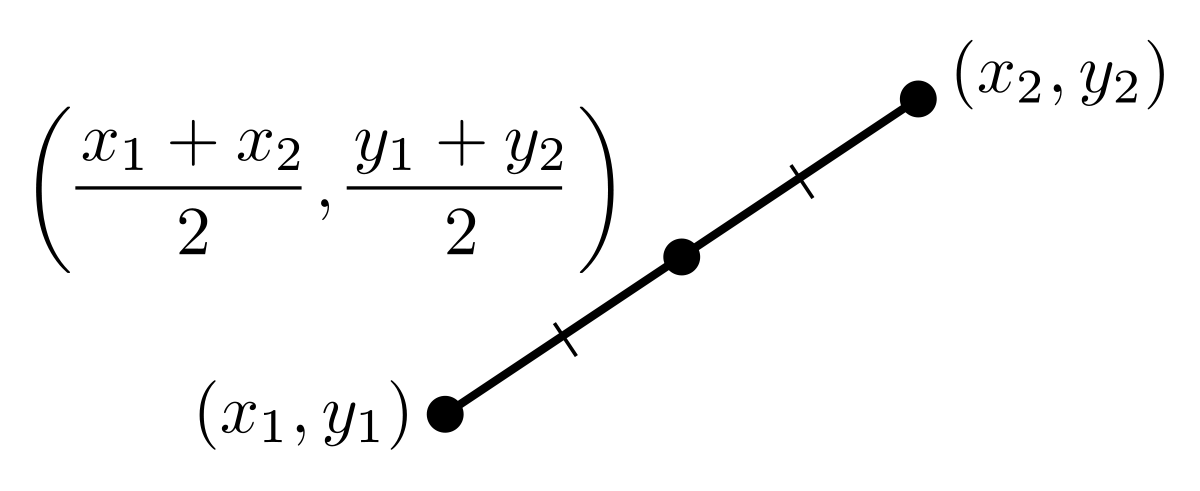
\includegraphics[width=2.60417in,height=\textheight]{img/middle_point.png}
\caption{punto medio}
\end{figure}

\hypertarget{cuxf3mo-calcularla}{%
\subsubsection{Cómo calcularla}\label{cuxf3mo-calcularla}}

Para calcularlo, si tenemos una tabla de frecuencias

\begin{longtable}[]{@{}ll@{}}
\toprule
\(x_i\) & \(n_i\)\tabularnewline
\midrule
\endhead
\(x_1\) & \(n_1\)\tabularnewline
\(x_2\) & \(n_2\)\tabularnewline
\(x_3\) & \(n_3\)\tabularnewline
\(\vdots\) & \(\vdots\)\tabularnewline
\(x_N\) & \(n_N\)\tabularnewline
\bottomrule
\end{longtable}

puesto que cada valor \(x_i\) se repite \(n_i\) veces, calcularemos la
media de la siguiente manera

\[\overline x = \frac{x_1 \cdot n_1 + x_2  \cdot n_2 + x_3  \cdot n_3 +\ldots  + x_N  \cdot n_N}{N} = \frac{1}{N}\sum^{N}_{i=1} x_i  \cdot n_i\]

en el caso de que tengamos una tabla de frecuencias agrupadas por
intervalos

\begin{longtable}[]{@{}lll@{}}
\toprule
\(I_i\) & \(x_i = \frac{x_i + x_{i+1}}{2}\) & \(n_i\)\tabularnewline
\midrule
\endhead
\([l_1, l_2)\) & \(x_1\) & \(n_1\)\tabularnewline
\([l_2, l_3)\) & \(x_2\) & \(n_2\)\tabularnewline
\([l_3, l_4)\) & \(x_3\) & \(n_3\)\tabularnewline
\(\vdots\) & \(\vdots\) & \(\vdots\)\tabularnewline
\([l_{K}, l_{K+1})\) & \(x_K\) & \(n_K\)\tabularnewline
\bottomrule
\end{longtable}

haremos lo mismo pero usando la marca de clase
\(x_i = \frac{l_i + l_{i+1}}{2}\)

\hypertarget{ejemplos}{%
\subsubsection{Ejemplos}\label{ejemplos}}

La siguiente tabla recoge las ventas de 100 sucursales de una empresa

\begin{longtable}[]{@{}llll@{}}
\toprule
ventas (miles) & \(x_i\) & \(n_i\) & \(x_i \cdot n_i\)\tabularnewline
\midrule
\endhead
{[}700, 800) & 750 & 4 & 3000\tabularnewline
{[}800, 900) & 850 & 7 & 5950\tabularnewline
{[}900, 1000) & 950 & 8 & 7600\tabularnewline
{[}1000, 1100) & 1050 & 10 & 10500\tabularnewline
{[}1100, 1200) & 1150 & 12 & 13800\tabularnewline
{[}1200, 1300) & 1250 & 17 & 21250\tabularnewline
{[}1300, 1400) & 1350 & 13 & 17550\tabularnewline
{[}1400, 1500) & 1450 & 10 & 14500\tabularnewline
{[}1500, 1600) & 1550 & 9 & 13950\tabularnewline
{[}1600, 1700) & 1650 & 7 & 11550\tabularnewline
{[}1700, 1800) & 1750 & 2 & 3500\tabularnewline
{[}1800, 1900) & 1850 & 1 & 1850\tabularnewline
\bottomrule
\end{longtable}

calculemos la media

\begin{align*}
\overline x &= \frac{1}{N}\sum^{N}_{i=1} x_i  \cdot n_i\\
&= \frac{750  \cdot  4 + 850  \cdot  7 + 950 \cdot 8 +  \ldots + 1850 \cdot  1}{100}\\
& = \frac{3000  + 5950  + 7600  + 10500 + 13800 + 21250 + 17550 + 14500 + 13950 + 11550 + 3500  + 1850}{100}\\
&=\frac{125000}{100}=1250
\end{align*}

\hypertarget{propiedades-de-la-media}{%
\subsubsection{Propiedades de la media}\label{propiedades-de-la-media}}

\begin{itemize}
\item
  Se ve muy afectada por valores extremos
\item
  La media de dos variables es la suma de dos medias

  \begin{align*}
   x_1, x_2, x_3,\ldots , x_n &\longrightarrow \overline x\\
   y_1, y_2, y_3,\ldots , y_n &\longrightarrow \overline y
   &\\
   x_1 + y_1, x_2+y_2, \ldots , x_n + y_n & \longrightarrow \overline{x+y}
  \end{align*}

  \[\overline{x + y} = \overline x + \overline y\]
\item
  Sumar a cada valor de los datos una cierta cantidad y hacer la media
  del resultado es lo mismo que sumar dicha cantidad a la media de los
  datos:
\end{itemize}

\begin{align*}
\overline{x+k} &= \frac{(x_1 +k)+ (x_2+k) +\ldots  + (x_N +k) }{N}\\
&=\frac{N\cdot k + x_1+  x_2 +  x_3  +\ldots  +  x_N}{N} = \overline {x} +k
\end{align*}

\begin{itemize}
\tightlist
\item
  Multiplicar a una variable por una cantidad y hacer su media resulta
  en multiplicar a la media por dicha cantidad:
\end{itemize}

\begin{align*}
k \overline{x} &= k\frac{x_1+ x_2  + x_3  +\ldots  + x_N }{N}\\
&=\frac{k x_1+ k x_2 + k x_3  +\ldots  + k x_N}{N} = \overline {kx}
\end{align*}

\hypertarget{moda}{%
\subsection{Moda}\label{moda}}

La \textbf{moda} (\(Mo\)) es el valor que aparece con mayor frecuencia
en un conjunto de datos. Si hubiera varios datos con frecuencia máxima
(no hay un único dato con mayor frecuencia sino varios) la moda serían
todos ellos. Por lo tanto la moda puede no ser única.

\hypertarget{cuxf3mo-calcularla-1}{%
\subsubsection{Cómo calcularla}\label{cuxf3mo-calcularla-1}}

Simplemente buscamos el valor o valores con mayor frecuencia absoluta.

\hypertarget{ejemplo-2}{%
\subsubsection{Ejemplo}\label{ejemplo-2}}

La siguente muestra es el resultado realizar una muestra de renta per
capita en un barrio concreto de madrid (en miles de euros anuales
brutos)

\[ 14, 23, 15, 17,12, 0.5, 30, 12, 23, 18, 25, 30, 15, 12, 23 \]

\begin{longtable}[]{@{}ll@{}}
\toprule
\(x_i\) & \(n_i\)\tabularnewline
\midrule
\endhead
0.5 & 1\tabularnewline
12 & 3\tabularnewline
14 & 1\tabularnewline
17 & 1\tabularnewline
18 & 1\tabularnewline
23 & 3\tabularnewline
30 & 2\tabularnewline
\bottomrule
\end{longtable}

Luego la moda es: \[Mo = 12, 23\]

\hypertarget{mediana}{%
\subsection{Mediana}\label{mediana}}

La mediana \(Me\) representa el valor de la variable de posición central
en un conjunto de datos ordenados.

Si tenemos un número impar de datos, tomamos como mediana simplemente el
valor que ocupe la posición central al ordenarlos, por ejemplo para los
datos

\[1, 2, 3, 4, 5\]

El dato central es \(3\) así que \(Me = 3\).

Si tenemos un número par de datos, al ordenar los datos no encontraremos
un dato central, sino dos, con lo cual tomaremos como mediana la media
entre estos dos datos centrales. Por ejemplo para los datos

\[7, 8, 9, 10, 11, 12 \]

No hay un dato central, podríamos decir que los valores \(9\) y \(10\)
son \emph{centrales} así que tomamos \(Me= (9+10)/2\)

\hypertarget{cuxf3mo-calcularla-2}{%
\subsubsection{Cómo calcularla}\label{cuxf3mo-calcularla-2}}

Si los datos no están en una tabla de frecuencias, haremos lo que hemos
comentado en los párrafos anteriores. Si hemos organizado los datos por
frecuencias, haremos lo siguiente:

Dada una tabla (en la que calculamos tambíen las frecuencias acumuladas)

\begin{longtable}[]{@{}lll@{}}
\toprule
\(x_i\) & \(n_i\) & \(N_i\)\tabularnewline
\midrule
\endhead
\(x_1\) & \(n_1\) & \(N_1\)\tabularnewline
\(x_2\) & \(n_2\) & \(N_2\)\tabularnewline
\(x_3\) & \(n_3\) & \(N_3\)\tabularnewline
\(\vdots\) & \(\vdots\) & \(\vdots\)\tabularnewline
\(x_N\) & \(n_N\) & \(N_N\)\tabularnewline
\bottomrule
\end{longtable}

\begin{enumerate}
\def\labelenumi{\arabic{enumi}.}
\tightlist
\item
  Buscamos el valor que ocupa la \emph{posición central} mirando en la
  tabla cual es el primer dato \(x_i\) cuya frecuencia acumulada supera
  o iguala \(N/2\).
\item
  Si encontramos un dato cuya frecuencia acumulada \(N_i\)
  \textbf{iguala} \(N/2\) tomamos como mediana la media de ese dato
  \(x_i\) y el siguiente \(x_{i+1}\). \(Me = \frac{x_{i} + x_{i+1}}{2}\)
\item
  Si no encontramos uno cuya \(N_i\) iguale a \(N/2\) sino uno que la
  supere directamente, tomamos ese dato como mediana. \(Me = x_i\).
\end{enumerate}

\hypertarget{ejemplo-1-1}{%
\subsubsection{Ejemplo 1}\label{ejemplo-1-1}}

Se recogen datos de la satisfacción de 37 usuarios con un servicio. Los
usuarios responden con notas del 1 al 9.

\begin{longtable}[]{@{}lll@{}}
\toprule
nota & \(n_i\) & \(N_i\)\tabularnewline
\midrule
\endhead
1 & 2 & 2\tabularnewline
2 & 2 & 4\tabularnewline
3 & 4 & 8\tabularnewline
4 & 5 & 13\tabularnewline
5 & 8 & 21\tabularnewline
6 & 9 & 30\tabularnewline
7 & 3 & 33\tabularnewline
8 & 4 & 37\tabularnewline
9 & 2 & 39\tabularnewline
\bottomrule
\end{longtable}

Calculamos \(N/2\) y obtenemos \(39/2 = 19.5\). Encontramos que el la
primera frecuencia acumulada que supera o iguala \(19.5\) es 21, no
habiendo ninguna que la iguale, de modo que \(Me = 5\)

\hypertarget{ejemplo-2-1}{%
\subsubsection{Ejemplo 2}\label{ejemplo-2-1}}

Si en el ejemplo anterior en lugar de la tabla anterior hubieramos
tenido la tabla:

\begin{longtable}[]{@{}lll@{}}
\toprule
nota & \(n_i\) & \(N_i\)\tabularnewline
\midrule
\endhead
1 & 2 & 2\tabularnewline
2 & 2 & 4\tabularnewline
3 & 4 & 8\tabularnewline
4 & 5 & 13\tabularnewline
5 & 8 & 21\tabularnewline
6 & 9 & 30\tabularnewline
7 & 3 & 33\tabularnewline
8 & 4 & 37\tabularnewline
9 & 5 & 42\tabularnewline
\bottomrule
\end{longtable}

En este caso \(N/2= 21\) y al mirar entre las frecuencias acumuladas
vemos que hay una que iguala 21, luego la mediana será
\[Me = (5+6)/2 = 5.5\]

\hypertarget{propiedades-de-la-mediana}{%
\subsubsection{Propiedades de la
mediana}\label{propiedades-de-la-mediana}}

\begin{itemize}
\tightlist
\item
  No se ve afectada por valores extremos.
\item
  Al igual que con la media \[Me(k\cdot x) = Me(x) \cdot k\]
  \[Me(k+ x) = Me(x) + k\] Esto se debe a que sumar todos los datos por
  una cantidad o multiplicarlos no varía la elección del valor central.
\item
  la mediana de la suma de dos conjuntos de datos (variables)
  \textbf{no} coincide con la suma de las medianas de estos datos.
\end{itemize}

\hypertarget{medidas-de-orden}{%
\section{Medidas de orden}\label{medidas-de-orden}}

Son medidas estadísticas que se basan en la ordenación de los datos para
extraer propiedades de la distribución.

Las principales medidas de orden son los Cuartiles y los percentiles.

\hypertarget{cuartiles-y-percentiles}{%
\subsection{Cuartiles y percentiles}\label{cuartiles-y-percentiles}}

Dados unos datos:

\[x_1, x_2, x_3,\ldots , x_n\]

\begin{itemize}
\tightlist
\item
  Dado cualquier número \(k\) entre 0 y 100, el \textbf{percentil} \(k\)
  (denotado por \(P_k\)) es el valor \(x_i\) de la muestra ordenada que
  deja tras de si al \(k\%\) de los datos.
\item
  El \textbf{primer cuartil} \(Q_1\) es el dato \(x_i\) de la muestra
  ordenada que deja tras de si a una cuarta parte de los datos. Por lo
  tanto \(Q_1 = P_{25}\)
\item
  El \textbf{segundo cuartil} \(Q_2\) es el dato \(x_i\) de la muestra
  ordenada que deja tras de si a la mitad de los datos. Es decir el
  segundo cuartil es la mediana. \(Q_2 = Me = P_{50}\).
\item
  El \textbf{tercer cuartil} \(Q_3\) es el dato \(x_i\) de la muestra
  ordenada que deja tras de si a tres cuartas partes de los datos. Por
  lo tanto \(Q_3 = P_{75}\)
\end{itemize}

\hypertarget{cuxf3mo-calcularlos}{%
\subsubsection{Cómo calcularlos}\label{cuxf3mo-calcularlos}}

Dada una tabla (en la que calculamos tambíen las frecuencias acumuladas)

\begin{longtable}[]{@{}lll@{}}
\toprule
\(x_i\) & \(n_i\) & \(N_i\)\tabularnewline
\midrule
\endhead
\(x_1\) & \(n_1\) & \(N_1\)\tabularnewline
\(x_2\) & \(n_2\) & \(N_2\)\tabularnewline
\(x_3\) & \(n_3\) & \(N_3\)\tabularnewline
\(\vdots\) & \(\vdots\) & \(\vdots\)\tabularnewline
\(x_N\) & \(n_N\) & \(N_N\)\tabularnewline
\bottomrule
\end{longtable}

\begin{enumerate}
\def\labelenumi{\arabic{enumi}.}
\tightlist
\item
  Buscamos el valor que deja tras de si a la proporción de los datos que
  buscamos, si queremos calcular el percentil \(k\), calculamos el \(k\)
  por ciento de N (es decir \(N\cdot k /100\)). Después mirando en la
  tabla cual es el primer dato \(x_i\) cuya frecuencia acumulada supera
  o iguala ese valor.
\item
  Si encontramos un dato cuya frecuencia acumulada \(N_i\)
  \textbf{iguala} el porcentaje de \(N\) calculado antes, tomamos como
  \(P_k\) la media de ese dato \(x_i\) y el siguiente \(x_{i+1}\).
\item
  Si no encontramos uno cuya \(N_i\) iguale el pordentaje anterior sino
  uno que la supere directamente, tomamos ese dato \(P_k\).
\end{enumerate}

Como se puede observar es el mismo proceso que hicimos con la mediana
pero en vez de hacer \(N/2\) hacemos \(N/4\) para \(Q_1\) o \(3N/4\)
para \(Q_3\).

\hypertarget{ejemplos-1}{%
\subsubsection{Ejemplos}\label{ejemplos-1}}

La siguiente tabla recoge los datos del número de veces que un conjunto
de 20 encuestados consumen un determinado servicio a la semana

\begin{longtable}[]{@{}lll@{}}
\toprule
\(x_i\) & \(n_i\) & \(N_i\)\tabularnewline
\midrule
\endhead
1 & 2 & 2\tabularnewline
2 & 5 & 7\tabularnewline
3 & 5 & 12\tabularnewline
4 & 3 & 15\tabularnewline
5 & 3 & 18\tabularnewline
6 & 1 & 19\tabularnewline
7 & 1 & 20\tabularnewline
\bottomrule
\end{longtable}

Calculemos los cuartiles

\begin{itemize}
\item
  Calculamos \(25 \cdot N / 100 = 5\). Buscamos el primer valor cuya
  \(N_i\) es mayor o igual que 5. Encontramos que el 2 directamente
  tiene una frecuencia acumulada que supera y no hay ningún valor que lo
  iguala. Así que \(Q_1 = 2\).
\item
  Calculamos \(N/2 = 5\). Buscamos el primer valor cuya \(N_i\) es mayor
  o igual que 10. Encontramos que el 3 directamente tiene una frecuencia
  acumulada que supera y no hay ningún valor que lo iguala. Así que
  \(Q_2 = Me = 3\).
\item
  Calculamos \(75 N/100 = 15\). Buscamos el primer valor cuya \(N_i\) es
  mayor o igual que 15. Encontramos que el 4 tiene una frecuencia
  acumulada que iguala 15 así que \(Q_3 = P_{75} = (4+5)/2\).
\end{itemize}

Calculemos el percentil 90 \(P_{90}\). Para ello calculamos
\(0.90*N = 18\). Buscamos el primer valor cuya \(N_i\) es mayor o igual
que 18. Encontramos que el 5 tiene una frecuencia acumulada que iguala
18 así que \(P_{90} = (5+6)/2\).

\hypertarget{medidas-de-dispersiuxf3n}{%
\section{Medidas de dispersión}\label{medidas-de-dispersiuxf3n}}

Las medidas de dispersión tratan, a \textbf{través de diferentes
cálculos}, de arrojar un valor numérico que ofrezca información sobre el
grado de variabilidad de una variable. En otras palabras, las medidas de
dispersión valores numéricos que indican si una variable se mueve mucho,
poco, más o menos que otra.

\hypertarget{rango-y-rango-intercuartuxedlico}{%
\subsection{Rango y rango
intercuartílico}\label{rango-y-rango-intercuartuxedlico}}

Dada una muestra \[ x_1, x_2, \ldots , x_N\]

El \textbf{rango} se define como

\[R= Max - Min\] donde \(Max\) es el valor máximo de la muestra y
\(Min\) el valor mínimo

Por otra parte el \textbf{rango intercuartílico} de define como

\[RI =  Q_3 - Q_1\]

Donde \(Q_3\) es el tercer cuartil y \(Q_1\) el primer cuartil.

Ambas dan una idea de cual es la distancia entre los valores más
pequeños y los más grandes que toma la muestra.

\hypertarget{varianza-y-desviaciuxf3n-tuxedpica}{%
\subsection{Varianza y desviación
típica}\label{varianza-y-desviaciuxf3n-tuxedpica}}

Dada una muestra \[ x_1, x_2, \ldots , x_N\]

La \textbf{varianza} se define como

\[S^2 = \frac{1}{n}\big( (x_1 - \overline x)^2 + (x_2 - \overline x)^2 + \ldots + (x_N - \overline x)^2 \big)= \frac{1}{n}\sum^N_{i=1} (x_i - \overline x)^2\]

La idea detrás de la varianza es promediar cuanto se separa cada valor
del valor medio.

Esto se aprecia bien en la siguiente figura

\begin{figure}
\centering
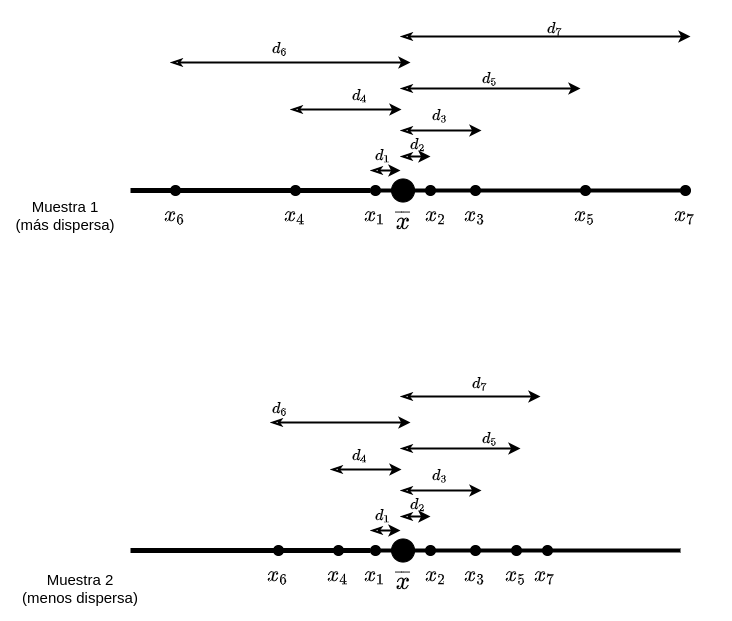
\includegraphics[width=5.72917in,height=\textheight]{img/desviaciones_diagrama.drawio.png}
\caption{~}
\end{figure}

En la figura vemos marcadas las distancias de cada punto respencto a la
media. La varianza no es sino las sumas de los cuadrados de esas
distancias. En la muestra 1 vemos como los datos están más separados
respecto a la media, de modo que esas distancias serán mayores, mientras
que en la muestra 2 (debajo) vemos como están menos separados y por lo
tanto esto impactará en las distancias. La muestra 1 de la figura tendrá
una varianza mayor que la muestra 2.

La varianza cumple que

\[S^2 = \overline{x^2} - \overline x^2\]

donde \(\overline{x^2}\) indica la media de los cuadrados de las
observaciones. Esta propiedad deduce simplemente expandiendo los
cuadrados \((x_i - \overline x)^2\) ya que:

\[S^2 = \frac{1}{n}\sum^N_{i=1} (x_i - \overline x)^2 = \frac{1}{n}\sum^N_{i=1} (x^2_i - 2x_i \overline x + \overline x^2)\]
\[=\frac{1}{n}\sum^N_{i=1} x_i^2 - \frac{1}{n}\sum^N_{i=1}2 x_i \overline x + \sum^N_{i=1}\overline x^2\]
\[=\frac{1}{n}\sum^N_{i=1} x_i^2 - 2 \overline x^2 + \overline x^2 = \frac{1}{n}\sum^N_{i=1} x_i^2 - \overline x^2 = \overline{x^2} - \overline x^2\]

La propiedad anterior permite en ocasiones calcular la varianza de una
forma más sencilla.

la desviación típica se define como la raíz cuadrada de la varianza:

\[S = \sqrt{(S^2)} = \sqrt{\frac{1}{n}\sum^N_{i=1} (x_i - \overline x)^2}\]

\hypertarget{cuxe1lculo-mediante-tablas-de-frecuencias}{%
\subsubsection{Cálculo mediante tablas de
frecuencias}\label{cuxe1lculo-mediante-tablas-de-frecuencias}}

Si tenemos una tabla de frecuencias

\begin{longtable}[]{@{}ll@{}}
\toprule
\(x_i\) & \(n_i\)\tabularnewline
\midrule
\endhead
\(x_1\) & \(n_1\)\tabularnewline
\(x_2\) & \(n_2\)\tabularnewline
\(x_3\) & \(n_3\)\tabularnewline
\(\vdots\) & \(\vdots\)\tabularnewline
\(x_N\) & \(n_N\)\tabularnewline
\bottomrule
\end{longtable}

puesto que cada valor de la tabla \(x_i\) se repite \(n_i\) veces
tenemos que modificar la formula anterior de la varianza para tener en
cuenta al sumar estas frecuencias.

Con una tabla como la anterior la varianza se calcula usando

\[S^2 = \frac{1}{n}\big( (x_1 - \overline x)^2 \cdot n_1 + (x_2 - \overline x)^2 \cdot n_2 + \ldots + (x_N - \overline x)^2 \cdot n_N \big)= \frac{1}{n}\sum^N_{i=1} (x_i - \overline x)^2 \cdot n_i\]

y la desviación tipica haciendo la raíz cuadrada de la expresión
anterior.

\[S = \sqrt{S^2}\]

Si deseamos usar la formula \(S^2 = \overline{x^2} - \overline x^2\)
debemos tener en cuenta que al tener los datos en una tabla de
frecuencias el valor \(\overline{x^2}\) se calculará usando:

\[\overline{x^2} = \sum^N_{i=1} x^2_i \cdot n_i\]

Esto lo veremos más claramente en el ejemplo más adelante. El proceso
será el mismo si tenemos una tabla agrupada por intervalos, simplemente
usaremos las marcas de clase.

\hypertarget{desviaciuxf3n-media}{%
\subsection{Desviación media}\label{desviaciuxf3n-media}}

Dada una muestra \((x_i)\) como la anterior la desviación media se
define de un modo similar a la varianza, pero tomando valores absolutos
en vez de cuadrados:

\[DM = \frac{1}{n}\big( |x_1 - \overline x| + |x_2 - \overline x| + \ldots + |x_N - \overline x| \big)= \frac{1}{n}\sum^N_{i=1} |x_i - \overline x|\]

Al igual que con la varianza, si tenemos los datos organizados en una
tabla de frecuencias deberemos multiplicar a cada sumando por su
frecuencia, es decir debemos usar

\[DM = \frac{1}{n}\sum^N_{i=1} |x_i - \overline x| \cdot n_i\]

\hypertarget{ejemplos-2}{%
\subsection{Ejemplos}\label{ejemplos-2}}

Volviendo al ejemplo de la encuesta de satisfacción realizado a unos
usuarios de un servicio, teníamos la tabla:

\begin{longtable}[]{@{}lll@{}}
\toprule
\(x_i\) & \(n_i\) & \(N_i\)\tabularnewline
\midrule
\endhead
1 & 2 & 2\tabularnewline
2 & 5 & 7\tabularnewline
3 & 5 & 12\tabularnewline
4 & 3 & 15\tabularnewline
5 & 3 & 18\tabularnewline
6 & 1 & 19\tabularnewline
7 & 1 & 20\tabularnewline
\bottomrule
\end{longtable}

Dado que el valor máximo es 7 el el mínimo es 1 tenemos:

\[R=Max - Min = 7-1=6\]

Recordemos que habíamos calculado que los cuartiles eran \(Q_1 =2\) y
\(Q_3 = 4.5\).

Por lo tanto tenemos

\[RI= Q_3 - Q_1 = 4.5 -2 = 2.5\]

Para calcular la varianza debo calcular la media. Ampliaremos la tabla
para simplificar los cálculos

\begin{longtable}[]{@{}lllll@{}}
\toprule
\(x_i\) & \(n_i\) & \(N_i\) & \(x_i \cdot n_i\) &
\(x_i^2 \cdot n_i\)\tabularnewline
\midrule
\endhead
1 & 2 & 2 & 2 & 2\tabularnewline
2 & 5 & 7 & 10 & 20\tabularnewline
3 & 5 & 12 & 15 & 45\tabularnewline
4 & 3 & 15 & 12 & 48\tabularnewline
5 & 3 & 18 & 15 & 75\tabularnewline
6 & 1 & 19 & 6 & 36\tabularnewline
7 & 1 & 20 & 7 & 49\tabularnewline
\bottomrule
\end{longtable}

de modo que para calcular la media me basta sumar la tercera columna
entera y dividir entre 20, es decir

\[\overline x = (2+10+15+\ldots 7)/20 = 3.35\]

y para calcular la varianza voy a usar la fórmula
\(S^2 = \overline{x^2} - \overline x^2\)

para calcular \(\overline{x^2}\) basta sumar la última columna
correspondiente a \(x_i^2 \cdot n_i\) y dividir entre el número de datos
\(20\).

\[\overline x^2 = (2+20+45+\ldots 49)/20 = 275/20 = 13.75\]

De modo que

\[S^2 =\overline{x^2} - \overline x^2 = 13.75-3.35^2 = 2.5275\]

Para calcular la desviación típica simplemente calculamos la raíz
cuadrada

\[S= \sqrt{2.5275} \cong 1.58\]

Para calcular la desviación media, necesitamos una vez más completar la
tabla para calcular las diferencias \(|x_i - \overline x|\cdot n_i\)

\begin{longtable}[]{@{}lll@{}}
\toprule
\(x_i\) & \(n_i\) & \(|x_i - \overline x|\cdot n_i\)\tabularnewline
\midrule
\endhead
1 & 2 & 4.7\tabularnewline
2 & 5 & 6.75\tabularnewline
3 & 5 & 1.75\tabularnewline
4 & 3 & 1.95\tabularnewline
5 & 3 & 4.95\tabularnewline
6 & 1 & 2.65\tabularnewline
7 & 1 & 3.65\tabularnewline
\bottomrule
\end{longtable}

y la variación media será el resultado de sumar la tercera columna y
dividir entre 20.

\[DM \cong 26.39/20\cong 1.31\]

\hypertarget{gruxe1ficos-estaduxedsticos}{%
\section{Gráficos estadísticos}\label{gruxe1ficos-estaduxedsticos}}

Los gráficos estadísticos son gráficos que intentan de capturar de forma
visual la información estadística de un conjunto de datos.
Particularmente tratan de representar lo concentrados o dispersos que
están los datos, los valores más comunes o más centrales de la
distribución así como la simetría o asimetría de los datos.

\hypertarget{histogramas-y-poluxedgonos-de-frecuencias}{%
\subsection{Histogramas y polígonos de
frecuencias}\label{histogramas-y-poluxedgonos-de-frecuencias}}

Los \textbf{histogramas} son gráficos en el que en el eje \(X\)
colocamos cada valor de los datos (o intervalo si hemos agrupado por
intervalos) y colocamos una barra o segmento encima de cada uno de estos
valores que tiene la altura igual a la frecuencia de dicho valor o
intervalo.

por ejemplo si tenemos los datos del ejemplo anterior

\begin{longtable}[]{@{}ll@{}}
\toprule
\(x_i\) & \(n_i\)\tabularnewline
\midrule
\endhead
1 & 2\tabularnewline
2 & 5\tabularnewline
3 & 5\tabularnewline
4 & 3\tabularnewline
5 & 3\tabularnewline
6 & 1\tabularnewline
7 & 1\tabularnewline
\bottomrule
\end{longtable}

resulta en el siguiente histograma

\begin{figure}
\centering
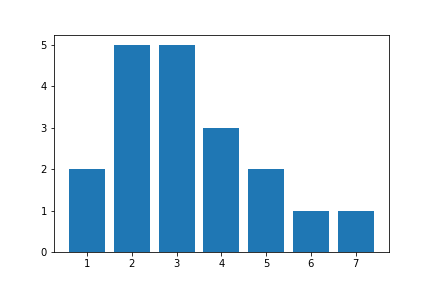
\includegraphics[width=3.64583in,height=\textheight]{img/histograma.png}
\caption{~}
\end{figure}

Mientras que para los datos

\begin{longtable}[]{@{}llll@{}}
\toprule
ventas (miles) & \(x_i\) & \(n_i\) & \(x_i \cdot n_i\)\tabularnewline
\midrule
\endhead
{[}700, 800) & 750 & 4 & 3000\tabularnewline
{[}800, 900) & 850 & 7 & 5950\tabularnewline
{[}900, 1000) & 950 & 8 & 7600\tabularnewline
{[}1000, 1100) & 1050 & 10 & 10500\tabularnewline
{[}1100, 1200) & 1150 & 12 & 13800\tabularnewline
{[}1200, 1300) & 1250 & 17 & 21250\tabularnewline
{[}1300, 1400) & 1350 & 13 & 17550\tabularnewline
{[}1400, 1500) & 1450 & 10 & 14500\tabularnewline
{[}1500, 1600) & 1550 & 9 & 13950\tabularnewline
{[}1600, 1700) & 1650 & 7 & 11550\tabularnewline
{[}1700, 1800) & 1750 & 2 & 3500\tabularnewline
{[}1800, 1900) & 1850 & 1 & 1850\tabularnewline
\bottomrule
\end{longtable}

Tendremos el histograma

\begin{figure}
\centering
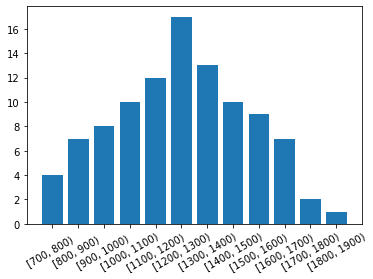
\includegraphics[width=3.64583in,height=\textheight]{img/histograma2.png}
\caption{~}
\end{figure}

Los \textbf{polígono de frecuencias} funcionan de forma muy similar a
los que los histogramas, pero en lugar de colocar barras, unimos con
segmentos los puntos que tienen en el eje \(X\) el valor de la muestra y
en el eje \(Y\) la frecuencia.

En el ejemplo anterior tenemos el siguiente \textbf{polígono de
frecuencias}

\begin{figure}
\centering
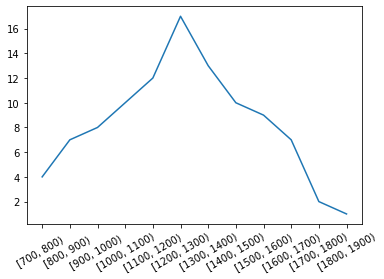
\includegraphics[width=3.64583in,height=\textheight]{img/diag_barras.png}
\caption{~}
\end{figure}

\hypertarget{propiedades-y-usos}{%
\subsubsection{Propiedades y usos}\label{propiedades-y-usos}}

\begin{itemize}
\tightlist
\item
  Tanto los histogramas y polígonos de frecuencias permiten visualizar
  la simetría de los datos. Permiten ver que valores o clases son más
  comunes o centrales de forma visual.
\item
  Como veremos, si estos diagramas tienen forma de \textbf{campana}
  suele significar que los datos siguen una distribución normal y esta
  información es muy valiosa.
\item
  Si las barras son muy caóticas y no se aprecia un valor central suele
  significar que los datos están \textbf{dispersos}
\end{itemize}

\hypertarget{diagramas-de-sectores}{%
\subsection{Diagramas de sectores}\label{diagramas-de-sectores}}

Los diagramas de sectores se basan en dividir una circunferencia en
tantos sectores como datos, intervalos o clases tengamos, de forma
proporcional a sus frecuencias.

por ejemplo si el dato \(x_i\) tiene frecuencia \(n_i\) dibujamos un
sector que tiene un ángulo de \(360\cdot n_i / N\) siendo \(N\) el
número de datos.

En el ejemplo anterior tendríamos

\begin{figure}
\centering
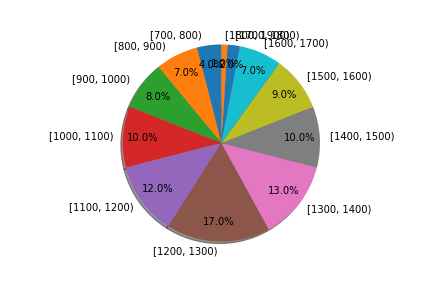
\includegraphics[width=3.64583in,height=\textheight]{img/sectores.png}
\caption{~}
\end{figure}

\hypertarget{propiedades-y-usos-1}{%
\subsubsection{Propiedades y usos}\label{propiedades-y-usos-1}}

\begin{itemize}
\tightlist
\item
  Son muy visuales y habitualmente agradables a la vista.
\item
  Tienen varios problemas: El orden de las clases (como se muestran en
  el circulo) es arbitrario, y eso puede dar lugar a confusión o
  interpretaciones erroneas.
\item
  El ojo humano tiene más problemas para diferenciar ángulos que
  longitudes, así que puede ser menos conveniente que otros.
\end{itemize}

\hypertarget{diagrama-de-cajas-y-bigotes}{%
\subsection{Diagrama de cajas y
bigotes}\label{diagrama-de-cajas-y-bigotes}}

Los \textbf{diagramas de cajas y bigotes} (también llamados boxplots).
Son una herramienta muy importante, que requiere un poco más de
conocimiento que los gráficos anteriores.

Si tenemos unos datos \(x_1, x_2, x_3,\ldots x_n\). Calculamos

\begin{itemize}
\tightlist
\item
  La Mediana \(Me\)
\item
  Los cuartiles \(Q_1\), \(Q_3\)
\item
  \(Min\), \(Max\)
\end{itemize}

Usamos estos datos para hacer un dibujo como el siguiente:

\begin{figure}
\centering
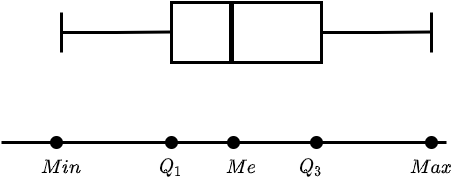
\includegraphics[width=3.64583in,height=\textheight]{img/boxplot.png}
\caption{~}
\end{figure}

\hypertarget{propiedades-y-usos-2}{%
\subsubsection{Propiedades y usos}\label{propiedades-y-usos-2}}

\hypertarget{bibliografuxeda}{%
\section{Bibliografía}\label{bibliografuxeda}}

\begin{itemize}
\tightlist
\item
  John A. Rice. Mathematical Statistics and Data Analysis
\item
  F. M. Dekking, C. Kraailkamp, H. P. Lopuhaa, L. E. Meester. A Modern
  Introduction to Probability and Statistics. Understanding Why and How.
\item
  \url{https://es.wikipedia.org/wiki/Distribuci\%C3\%B3n_Bernoulli}
\item
  \url{https://es.wikipedia.org/wiki/Distribuci\%C3\%B3n_binomial}
\item
  \url{https://es.wikipedia.org/wiki/Distribuci\%C3\%B3n_geom\%C3\%A9trica}
\end{itemize}

\end{document}